\documentclass[UTF8,a4paper,12pt,openany,fontset=fandol]{ctexrep}

\usepackage[a4paper,top=2.5cm,bottom=2.5cm,left=2.6cm,right=2.6cm,headheight=15pt]{geometry}
\usepackage{fontspec}
\usepackage{graphicx}
\usepackage{booktabs}
\usepackage{longtable}
\usepackage{array}
\usepackage{tabularx}
\usepackage{xcolor}
\usepackage{listings}
\usepackage{caption}
\usepackage{float}
\usepackage{pdflscape}
\usepackage{adjustbox}
\usepackage{enumitem}
\usepackage{fancyhdr}
\usepackage{setspace}
\usepackage{etoolbox}
\usepackage{chngcntr}
\usepackage{hyperref}

% Fandol is bundled with TeX Live and is the final free fallback on both
% Windows and Linux. To prefer a host font, replace fontset=fandol above with
% fontset=windows, or set Noto/Source Han here when those full families exist.
\setmonofont{Latin Modern Mono}

\definecolor{codebg}{RGB}{246,247,249}
\definecolor{codeframe}{RGB}{215,219,224}
\definecolor{codecomment}{RGB}{70,120,82}
\definecolor{codekeyword}{RGB}{38,76,150}
\definecolor{linkblue}{RGB}{20,75,135}
\definecolor{quotebg}{RGB}{247,249,252}
\definecolor{quoteedge}{RGB}{91,125,166}

\lstset{
  basicstyle=\small\ttfamily,
  backgroundcolor=\color{codebg},
  frame=single,
  rulecolor=\color{codeframe},
  framesep=5pt,
  xleftmargin=0.8em,
  xrightmargin=0.3em,
  breaklines=true,
  breakatwhitespace=false,
  keepspaces=true,
  columns=fullflexible,
  showstringspaces=false,
  tabsize=4,
  upquote=true,
  commentstyle=\color{codecomment},
  keywordstyle=\color{codekeyword},
  numbers=none,
  aboveskip=0.8em,
  belowskip=0.8em
}

\hypersetup{
  unicode=true,
  colorlinks=true,
  linkcolor=linkblue,
  urlcolor=linkblue,
  citecolor=linkblue,
  bookmarksnumbered=true,
  pdfstartview=FitH,
  pdftitle={操作系统课程设计报告},
  pdfauthor={张晓文}
}

\captionsetup{font=small,labelsep=space}
\captionsetup[figure]{name=图}
\captionsetup[table]{name=表}
\counterwithout{figure}{chapter}
\counterwithout{table}{chapter}
\renewcommand{\thefigure}{\arabic{figure}}
\renewcommand{\thetable}{\arabic{table}}
\setcounter{secnumdepth}{2}
\setcounter{tocdepth}{2}

\ctexset{
  chapter={
    format=\centering\heiti\zihao{2},
    name={第,章},
    number=\chinese{chapter},
    beforeskip=0pt,
    afterskip=24pt
  },
  section={
    format=\heiti\zihao{3},
    beforeskip=1.5ex,
    afterskip=0.8ex
  },
  subsection={
    format=\heiti\zihao{4},
    beforeskip=1.2ex,
    afterskip=0.6ex
  }
}

\setlength{\parindent}{2em}
\setlength{\parskip}{0.25em}
\setstretch{1.35}
\setlist{nosep,leftmargin=2.4em}
\setlength{\LTpre}{0.5em}
\setlength{\LTpost}{0.5em}
\renewcommand{\arraystretch}{1.25}
\emergencystretch=2em
\sloppy

\pagestyle{fancy}
\fancyhf{}
\fancyhead[C]{\small 操作系统课程设计报告}
\fancyfoot[C]{\small\thepage}
\renewcommand{\headrulewidth}{0.4pt}
\renewcommand{\footrulewidth}{0pt}

\newenvironment{reportquote}
  {\begin{quote}\small\color{quoteedge}}
  {\end{quote}}

\newcommand{\reportfigure}[3]{%
  \begin{figure}[H]
    \centering
    \includegraphics[width=#2\textwidth,height=0.72\textheight,keepaspectratio]{figures/#1}
    \caption{#3}
  \end{figure}
}

\begin{document}

\begin{titlepage}
  \thispagestyle{empty}
  \centering
  \vspace*{2.1cm}
  {\heiti\zihao{0} 操作系统课程设计报告\par}
  \vspace{1.5cm}
  {\heiti\zihao{2} 基于自研 RV64I 模拟平台的 MiniOS\\[0.35cm]
  操作系统设计与实现\par}
  \vfill
  \renewcommand{\arraystretch}{1.7}
  {\zihao{3}
  \begin{tabular}{>{\heiti}r l}
    学生姓名： & 张晓文 \\
    学\hspace{2em}号： & 20231071455 \\
  \end{tabular}\par}
  \vfill
  {\zihao{3}\mbox{2026 年 6 月}\par}
  \vspace*{1.5cm}
\end{titlepage}

\pagenumbering{Roman}
\tableofcontents
\clearpage
\pagenumbering{arabic}
\setcounter{page}{1}
\chapter{前言}

\section{项目背景}

操作系统课程设计要求从系统开发者视角出发，完成一个简化操作系统的设计与实现，重点理解系统启动、内核管理、进程调度、内存管理、文件系统、系统调用和用户程序运行机制。

本项目在前序体系结构课程设计的基础上继续扩展。前序课程中已经实现了一个自研 RISC-V RV64I 模拟器 \nolinkurl{cemu}，能够模拟 CPU、内存、总线和基础外设。操作系统课程设计中，本项目没有直接采用 QEMU，而是在该自研 RISC-V 平台上实现 MiniOS。这样既保持了两门课程之间的联动，也使操作系统能够在一个可控、可理解的硬件抽象环境中运行。

\section{项目目标}

本项目的目标是实现一个运行在 RISC-V RV64I 模拟平台上的教学型操作系统 MiniOS，具备以下能力：

\begin{enumerate}
\item 能够通过 Bootloader 完成两阶段启动。
\item 能够从 M 态切换到 S 态，并启动 S 态内核。
\item 支持 U 态用户程序运行，形成 M/S/U 三种特权级运行路径。
\item 支持 Sv39 虚拟内存机制和用户地址空间。
\item 支持进程创建、执行、退出、等待和调度。
\item 支持系统调用机制。
\item 支持持久化文件系统 MiniFS v2。
\item 支持独立 ELF 用户程序加载和运行。
\item 支持交互式 Shell，能够执行文件、目录、进程相关命令。
\item 能够通过系统运行测试证明上述功能形成闭环。
\end{enumerate}

\section{项目总体成果}

本项目最终形成了一个从模拟硬件到用户态程序的完整系统闭环：

\begin{lstlisting}
cemu 模拟平台
  -> boot.bin 第一阶段 Bootloader
  -> disk.img 中的 kernel.bin
  -> MiniOS S-mode Kernel
  -> MiniFS v2 文件系统
  -> ELF 用户程序
  -> C Shell 交互环境
\end{lstlisting}

系统已经能够启动到 Shell，支持执行 \nolinkurl{/bin} 下的命令和 \nolinkurl{/tests} 下的测试程序，并支持文件跨模拟器重启持久保存。

\chapter{技术方案设计}

\section{总体架构}

MiniOS 项目整体可以分为四层：

\begin{enumerate}
\item \textbf{宿主环境层}：项目运行在 WSL / Linux 环境中，通过 CMake、Makefile 和 RISC-V 裸机工具链完成构建。
\item \textbf{硬件模拟层}：由自研 \nolinkurl{cemu} 模拟器提供 RISC-V CPU、DRAM、CSR、MMU、Bus、UART、CLINT、PLIC 和 Block Device 等硬件抽象。
\item \textbf{MiniOS 内核层}：包括 Bootloader、内核启动、trap 处理、系统调用、物理页分配、虚拟内存、进程管理、调度器、文件系统和 ELF loader。
\item \textbf{用户程序层}：包括 C Shell、简化 libc、用户程序入口 \nolinkurl{crt0.S}、\nolinkurl{ls/cat/echo/pwd/ps/kill/mkdir/rm/touch/write} 等命令，以及 \nolinkurl{fstest/forktest/argtest/spin} 等测试程序。
\end{enumerate}

\begin{landscape}
\begin{figure}[H]
\centering
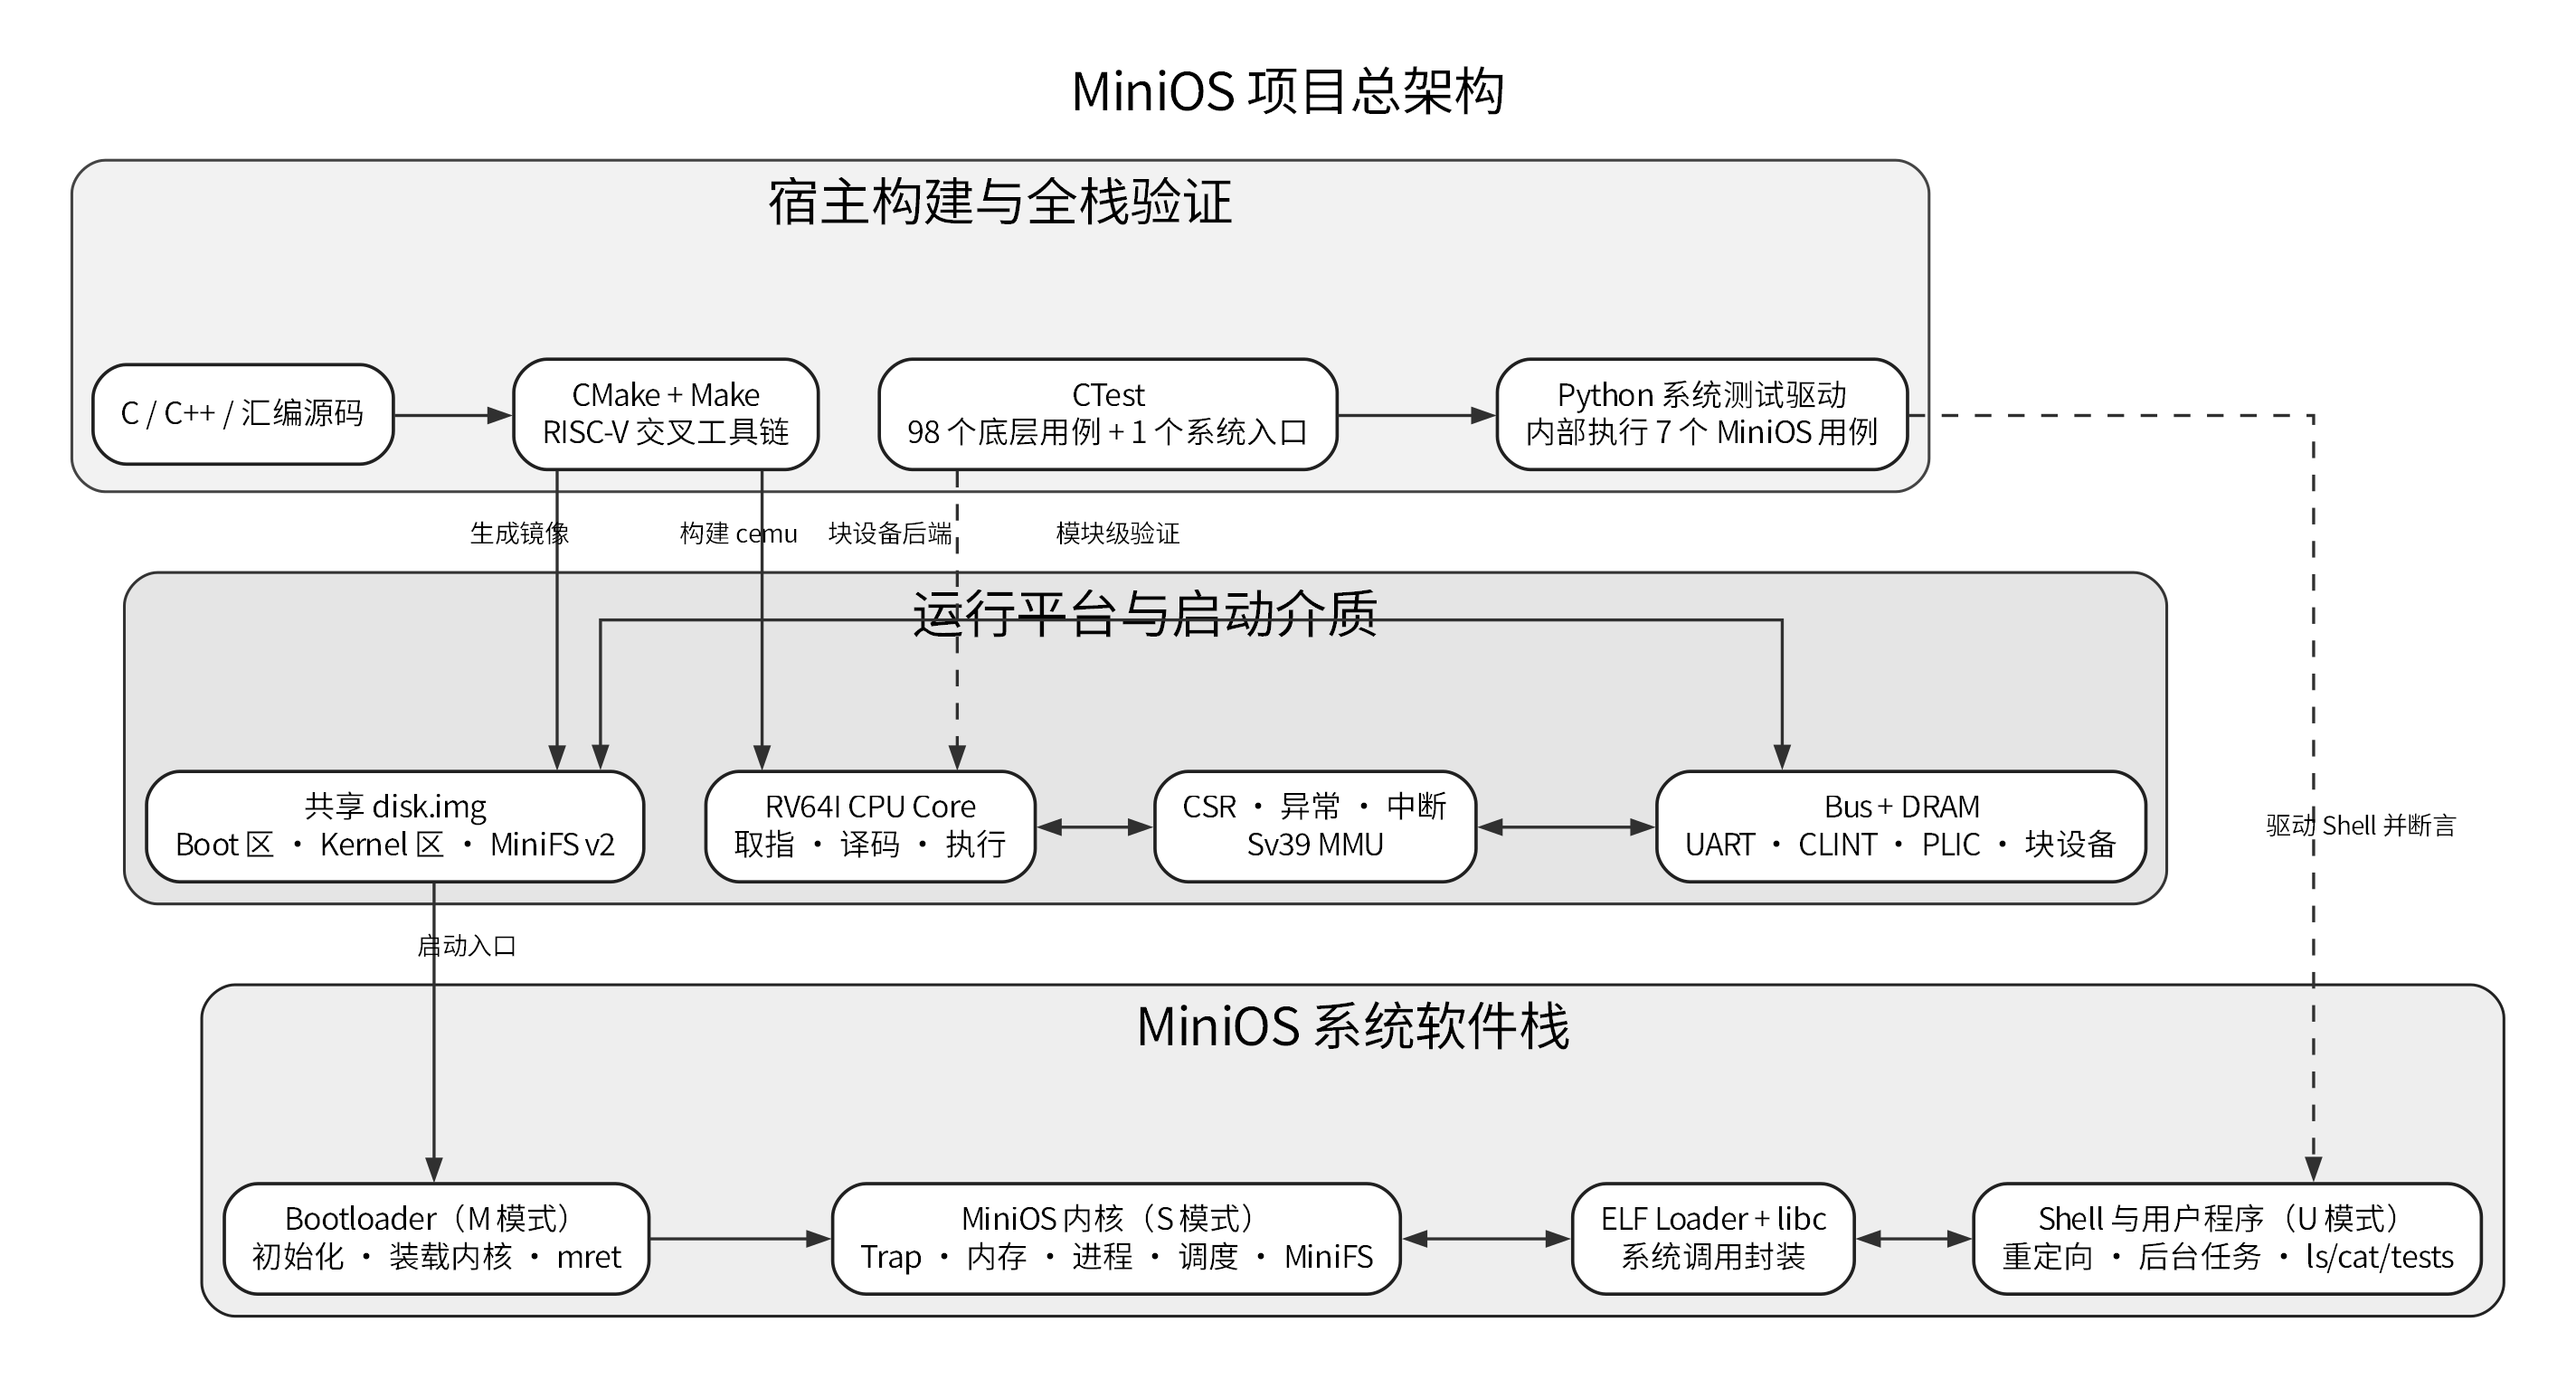
\includegraphics[width=0.94\linewidth,height=0.78\textheight,keepaspectratio]{figures/fig01_project_architecture.png}
\caption{MiniOS / myCPU 总体架构图}
\end{figure}
\end{landscape}

\section{技术选型}

本项目采用 RISC-V 架构，具体选择如下：

\begin{table}[H]
\centering
\small
\begin{adjustbox}{max width=\textwidth}
\begin{tabularx}{\textwidth}{>{\raggedright\arraybackslash}X>{\raggedright\arraybackslash}X}
\toprule
\textbf{项目} & \textbf{技术选型} \\
\midrule
指令集架构 & RISC-V RV64I \\
特权级 & M-mode / S-mode / U-mode \\
虚拟内存 & Sv39 \\
内核语言 & C + RISC-V 汇编 \\
用户程序语言 & C + RISC-V 汇编启动入口 \\
文件系统 & 自研 MiniFS v2 \\
用户程序格式 & ELF64 RISC-V 静态可执行文件 \\
调度算法 & RR 为主，支持 FCFS \\
运行平台 & 自研 \nolinkurl{cemu} RV64I 模拟器 \\
构建工具 & CMake + Makefile \\
测试方式 & CTest 单元测试 + MiniOS 系统级运行测试 \\
\bottomrule
\end{tabularx}
\end{adjustbox}
\end{table}

\section{cemu 模拟平台简介}

\nolinkurl{cemu} 是本项目的运行平台，提供 MiniOS 所需的基本硬件抽象。其核心模块包括：

\begin{table}[H]
\centering
\small
\begin{adjustbox}{max width=\textwidth}
\begin{tabularx}{\textwidth}{>{\raggedright\arraybackslash}X>{\raggedright\arraybackslash}X}
\toprule
\textbf{模块} & \textbf{作用} \\
\midrule
CPU Core & 维护 PC、通用寄存器、当前特权级，完成取指、译码和执行 \\
CSR & 提供控制状态寄存器，支持异常、中断和特权级控制 \\
MMU & 实现 Sv39 地址翻译和权限检查 \\
Bus & 根据物理地址进行 MMIO 路由 \\
DRAM & 提供 128 MiB 主存 \\
UART & 提供终端输入输出 \\
CLINT & 提供定时器与 \nolinkurl{mtime/mtimecmp} \\
PLIC & 提供平台级外部中断控制 \\
Block Device & 提供 8 MiB 持久化块设备 \nolinkurl{disk.img} \\
\bottomrule
\end{tabularx}
\end{adjustbox}
\end{table}

\nolinkurl{cemu} 的模块关系可以概括为：

\begin{lstlisting}
main.cpp
  -> Cpu
      -> MMU
      -> CSR
      -> Bus
          -> DRAM
          -> UART
          -> CLINT
          -> PLIC
          -> BlockDevice
      -> Exception
\end{lstlisting}

\begin{landscape}
\begin{figure}[H]
\centering
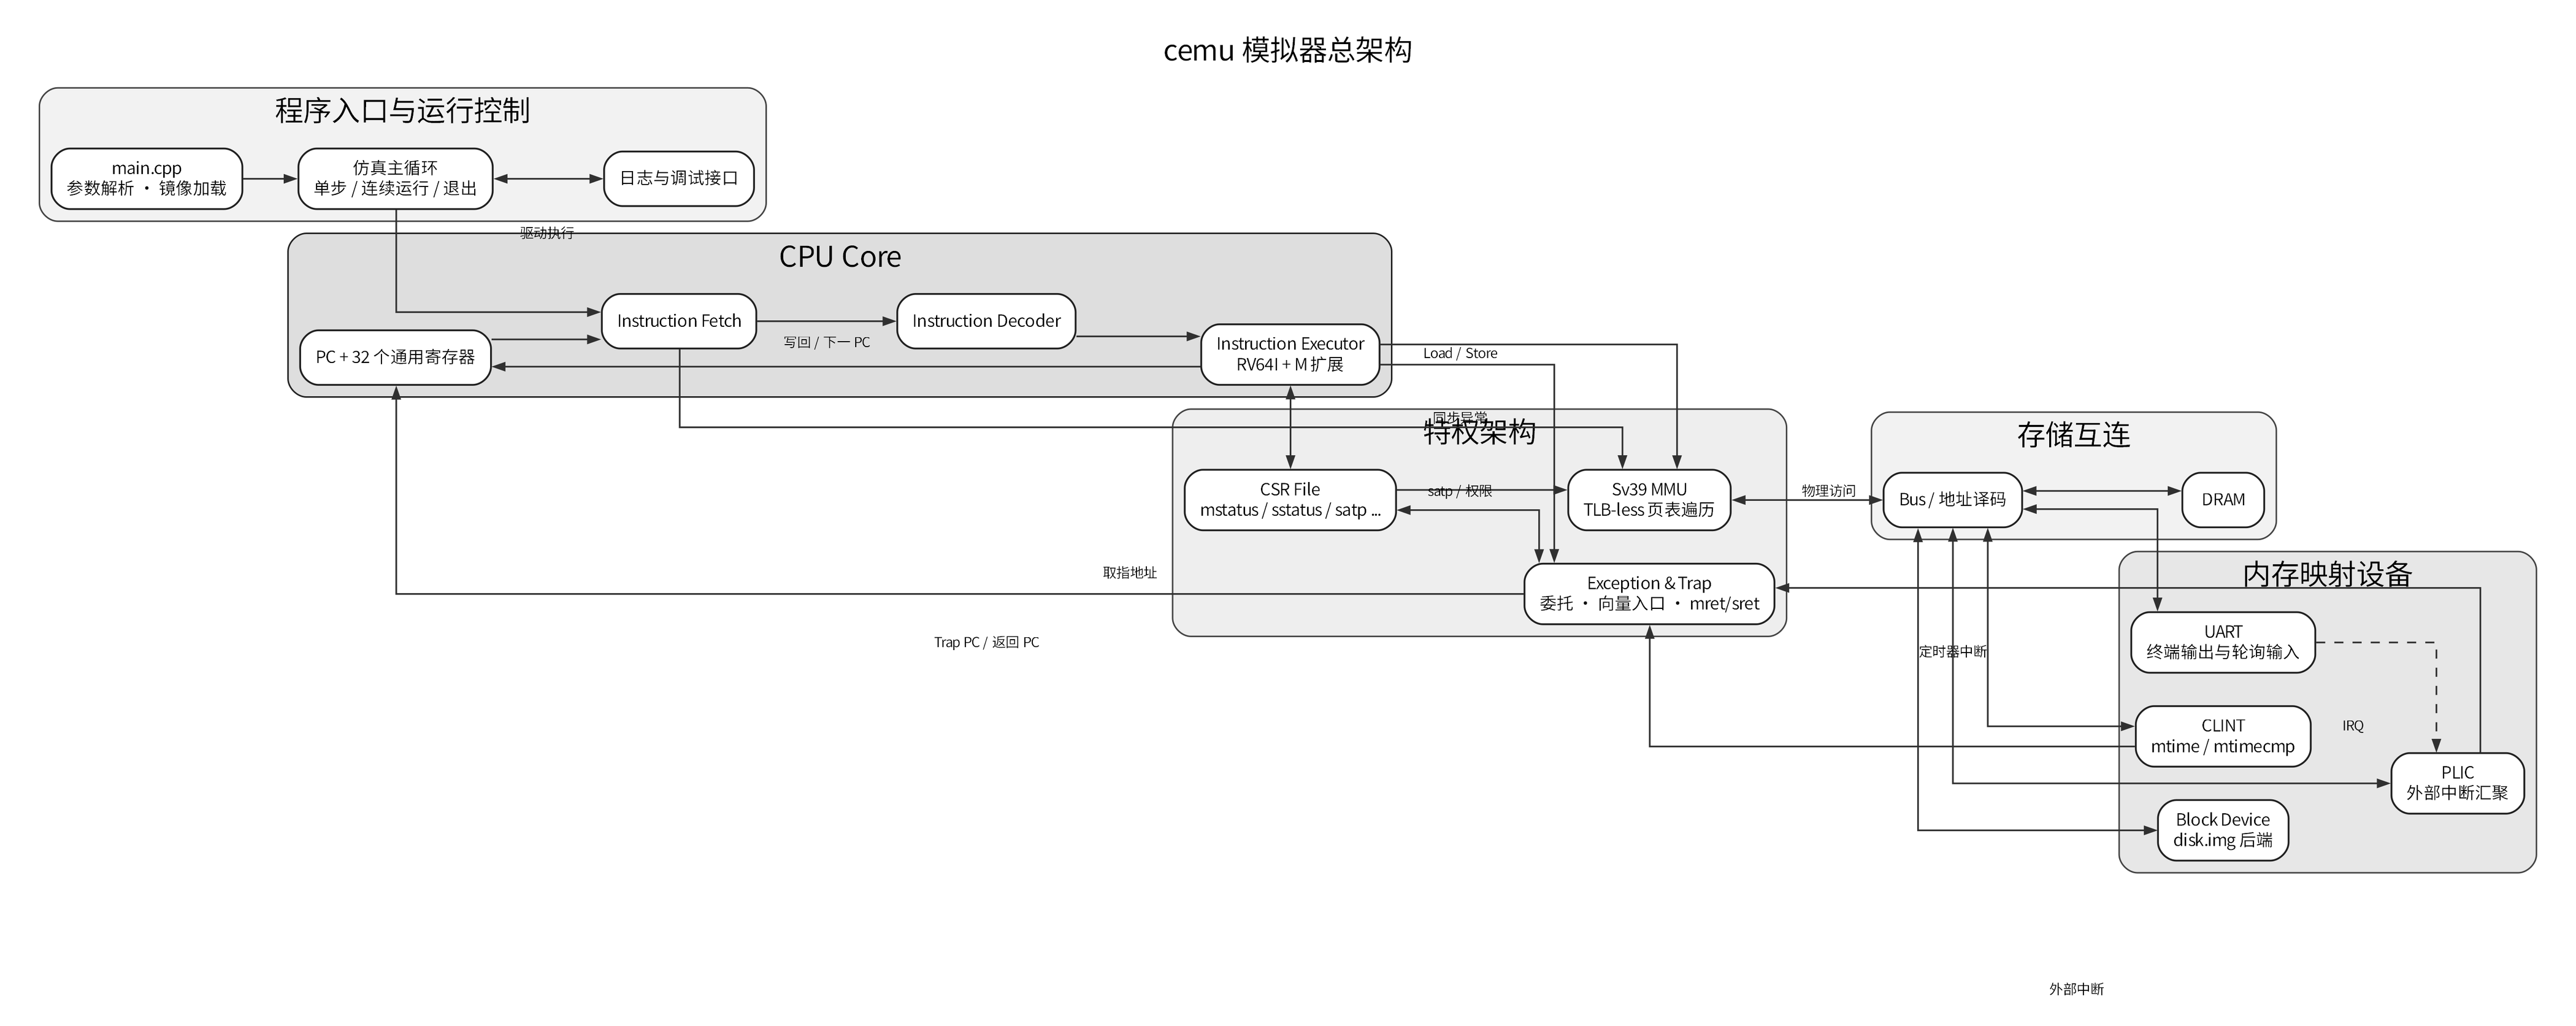
\includegraphics[width=0.94\linewidth,height=0.78\textheight,keepaspectratio]{figures/fig02_simulator_architecture.png}
\caption{cemu 模拟器结构图}
\end{figure}
\end{landscape}

\section{单条指令执行流程}

在模拟器主循环中，每条指令大致经历以下过程：

\begin{enumerate}
\item 检查系统是否已经停机。
\item 推进 CLINT 定时器。
\item 检查是否存在待处理的中断。
\item 根据 PC 取指。
\item MMU 根据当前特权级和页表状态进行地址翻译。
\item Bus 从对应物理地址读取指令。
\item 指令执行器根据 opcode / funct3 / funct7 完成译码。
\item 执行 ALU、访存、跳转、CSR 或异常相关操作。
\item 更新 PC。
\item 若发生异常或中断，则进入异常处理流程，设置 EPC、CAUSE、TVAL 和 TVEC，并切换到对应 trap 入口。
\end{enumerate}

\begin{landscape}
\begin{figure}[H]
\centering
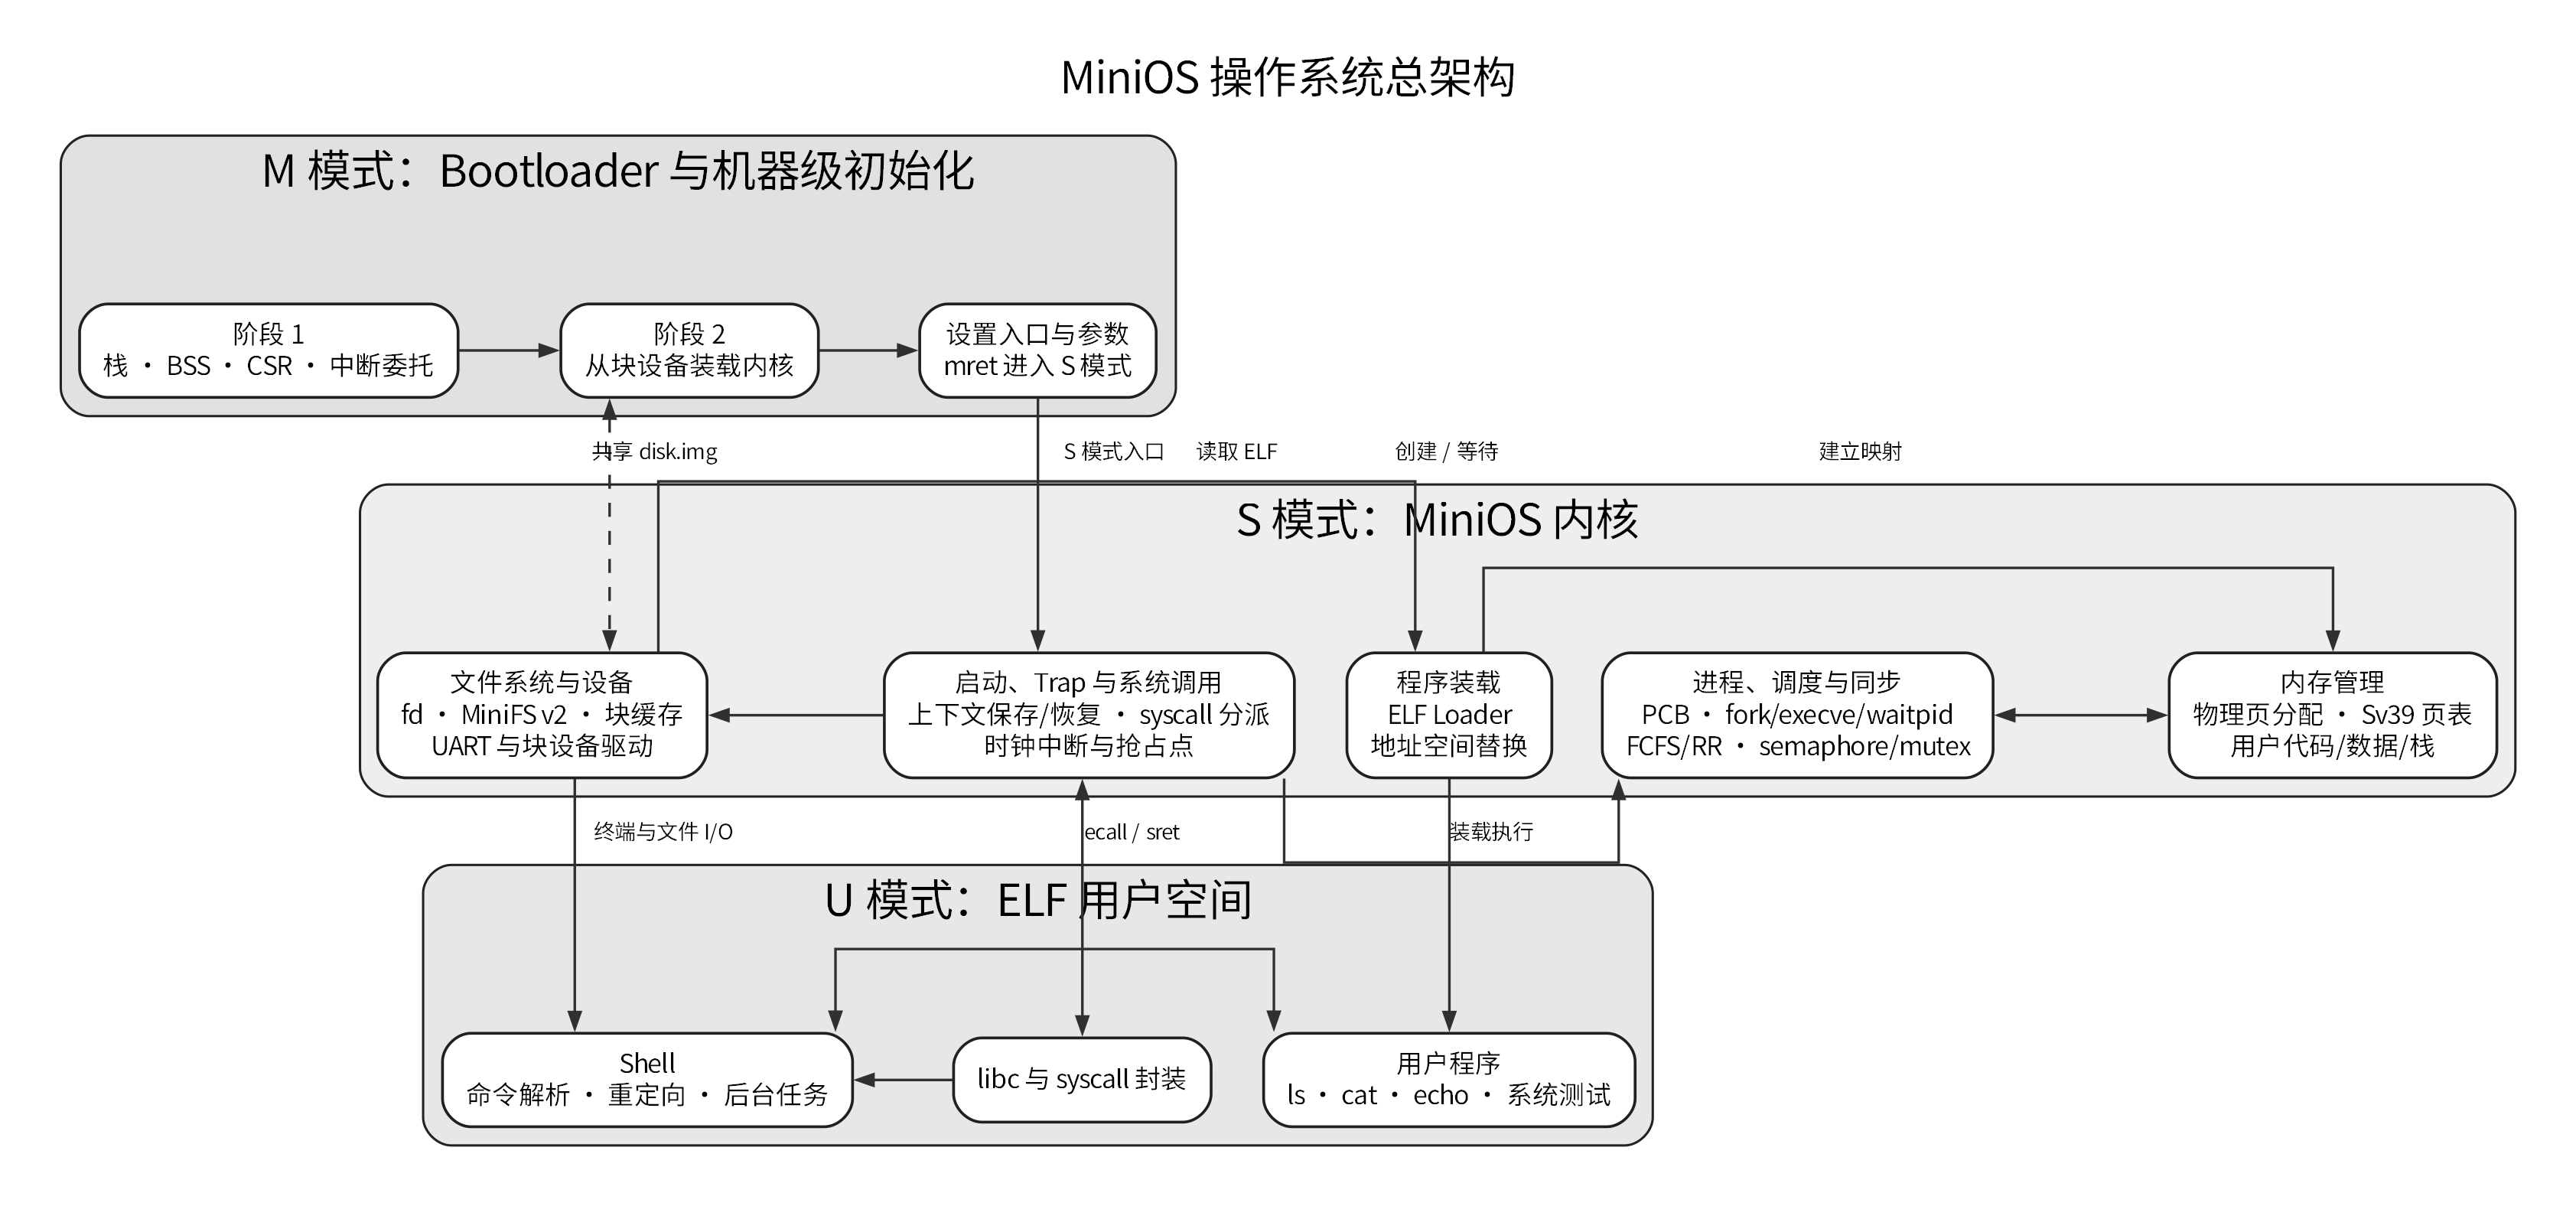
\includegraphics[width=0.94\linewidth,height=0.78\textheight,keepaspectratio]{figures/fig03_os_architecture.png}
\caption{CPU 单指令执行流程图}
\end{figure}
\end{landscape}

\begingroup
\let\clearpage\relax
\chapter{系统启动模块}
\endgroup

\section{设计目标}

启动模块的目标是让 MiniOS 不再依赖模拟器直接加载内核，而是通过真实的两阶段启动链路完成系统启动。这样可以更接近真实操作系统的启动方式，也能体现 Bootloader、块设备、镜像校验和内核入口之间的关系。

\section{两阶段启动流程}

MiniOS 当前使用如下启动链路：

\begin{lstlisting}
cemu
  -> 仅加载 boot.bin 到 0x80000000
  -> CPU 从 0x80000000 以 M 态执行
  -> Bootloader 读取 disk.img 尾部内核槽
  -> 校验内核镜像头
  -> 读取 kernel.bin
  -> 计算 checksum
  -> 搬运内核到 0x80200000
  -> 跳转到内核 _start
  -> 内核设置栈、清零 BSS、初始化 trap 向量
  -> mret 从 M 态进入 S 态 kernel_main
  -> 初始化 MiniOS 子系统
  -> 启动用户 Shell
\end{lstlisting}

\section{Bootloader 镜像加载}

Bootloader 位于 \nolinkurl{0x80000000}，内核加载地址为 \nolinkurl{0x80200000}。磁盘布局中，前部为 MiniFS 文件系统，尾部保留为内核槽：

\begin{table}[H]
\centering
\small
\begin{adjustbox}{max width=\textwidth}
\begin{tabularx}{\textwidth}{>{\raggedright\arraybackslash}X>{\raggedright\arraybackslash}X}
\toprule
\textbf{扇区} & \textbf{用途} \\
\midrule
0-15359 & MiniFS v2 文件系统区域 \\
15360 & 64 B 内核镜像头 \\
15361-16383 & \nolinkurl{kernel.bin} 裸二进制镜像 \\
\bottomrule
\end{tabularx}
\end{adjustbox}
\end{table}

内核镜像头包含 magic、版本号、头长度、加载地址、入口地址、镜像大小和 checksum。Bootloader 会在跳转前完成校验，若校验失败则停止执行，避免损坏内核被加载。

\nolinkurl{os/boot/loader.c} 中的核心校验与跳转逻辑如下：

\begin{lstlisting}[language=c]
if (!bytes_equal(header->magic, expected_magic, sizeof(expected_magic)))
    boot_fail("bad kernel magic");
if (header->version != BOOT_IMAGE_VERSION ||
    header->header_size != BOOT_IMAGE_HEADER_SIZE)
    boot_fail("unsupported kernel image");
if (header->load_address != KERNEL_LOAD_ADDRESS)
    boot_fail("unexpected load address");
/* 逐扇区复制时累加 checksum */
if (checksum != expected_checksum)
    boot_fail("checksum mismatch");
void (*kernel_entry)(void) = (void (*)(void))(uintptr_t)entry;
kernel_entry();
\end{lstlisting}

\section{M 态到 S 态切换}

内核 \nolinkurl{_start} 入口运行在 M 态。启动代码完成以下工作：

\begin{enumerate}
\item 初始化内核栈。
\item 清零 BSS。
\item 设置 M 态 trap 向量。
\item 设置 S 态 trap 向量。
\item 配置异常和中断委托。
\item 设置 \nolinkurl{mstatus.MPP = S}。
\item 设置 \nolinkurl{mepc = kernel_main}。
\item 执行 \nolinkurl{mret} 进入 S 态内核主函数。
\end{enumerate}

\nolinkurl{os/boot/start.S} 中的特权级切换代码如下：

\begin{lstlisting}
la t0, trap_entry
csrw stvec, t0
li t0, (1 << 11)       # mstatus.MPP = S
csrs mstatus, t0
la t0, kernel_main
csrw mepc, t0
mret
\end{lstlisting}

\section{启动模块小结}

启动模块实现了从模拟器预装 Bootloader，到 Bootloader 自主加载内核，再到内核切换 S 态并启动 Shell 的完整链路。该设计使 MiniOS 的启动过程更加接近真实操作系统，也降低了模拟器对内核加载过程的“代做”程度。

\reportfigure{fig04_boot.png}{0.55}{MiniOS 两阶段启动流程图}

\chapter{内存管理模块}

\section{物理内存布局}

MiniOS 运行在 128 MiB DRAM 上，主要内存布局如下：

\begin{table}[H]
\centering
\small
\begin{adjustbox}{max width=\textwidth}
\begin{tabularx}{\textwidth}{>{\raggedright\arraybackslash}X>{\raggedright\arraybackslash}X}
\toprule
\textbf{地址范围} & \textbf{用途} \\
\midrule
\nolinkurl{0x80000000-0x801fffff} & Bootloader 区域 \\
\nolinkurl{0x80200000-...} & MiniOS 内核镜像与 BSS \\
中间区域 & 物理页分配区 \\
\nolinkurl{0x87fc0000-0x87ffffff} & 内核栈保护区 \\
\nolinkurl{0x88000000} & 内核初始栈顶 \\
\bottomrule
\end{tabularx}
\end{adjustbox}
\end{table}

物理内存管理采用页级分配方式。内核初始化时建立可用物理页链表，后续内核页表、用户地址空间、用户栈和 ELF 段加载都通过页分配器获得物理页。

\section{页分配器设计}

MiniOS 实现了基于 4 KiB 页的物理页分配器。其主要职责包括：

\begin{enumerate}
\item 初始化可分配物理页范围。
\item 支持 \nolinkurl{kalloc} 分配物理页。
\item 支持 \nolinkurl{kfree} 回收物理页。
\item 维护空闲页链表。
\item 为内核页表、用户页表、用户程序加载和 fork 地址空间复制提供基础。
\end{enumerate}

\nolinkurl{os/kernel/mem.c} 采用“空闲链表优先、bump allocator 兜底”的页分配策略：

\begin{lstlisting}[language=c]
void *kalloc(void) {
    if (free_list != NULL) {
        struct free_page *page = free_list;
        free_list = page->next;
        total_free--;
        return (void *)page;
    }
    if (bump_ptr + PAGE_SIZE > heap_end)
        return NULL;
    void *page = (void *)bump_ptr;
    bump_ptr += PAGE_SIZE;
    total_free--;
    return page;
}

void kfree(void *ptr) {
    struct free_page *page = (struct free_page *)ptr;
    page->next = free_list;
    free_list = page;
    total_free++;
}
\end{lstlisting}

\section{Sv39 虚拟内存}

MiniOS 使用 RISC-V Sv39 虚拟内存机制。内核启动时建立内核页表，将 DRAM 和 MMIO 区域映射到内核地址空间。用户程序运行时拥有独立用户页表，内核通过页表权限实现用户态和内核态隔离。

Sv39 页表提供三级页表结构。虚拟地址经过 VPN[2]、VPN[1]、VPN[0] 三级索引找到页表项，再结合页内偏移形成物理地址。MMU 会根据页表项中的权限位检查当前访问是否合法。

\section{用户地址空间}

用户程序由 ELF loader 加载到用户地址空间中。每个用户进程拥有独立地址空间，主要包括：

\begin{enumerate}
\item ELF 代码段。
\item ELF 数据段。
\item BSS 区域。
\item 用户栈。
\item \nolinkurl{argc/argv/envp} 初始栈内容。
\end{enumerate}

\nolinkurl{fork} 时，MiniOS 会深复制父进程用户页，构造子进程地址空间。\nolinkurl{execve} 时，内核会先构造新的用户地址空间，成功后再原子替换旧地址空间。

\nolinkurl{os/kernel/user.c} 在 \nolinkurl{execve} 成功后才替换旧地址空间，并刷新 TLB：

\begin{lstlisting}[language=c]
struct task_address_space old_space;
if (task_replace_address_space(&program.space, &old_space) < 0) {
    user_space_destroy(&program.space);
    return -1;
}
csr_write(satp, program.space.satp);
__asm__ volatile("sfence.vma x0, x0");
user_space_destroy(&old_space);
trap_frame[2] = program.stack_pointer;
trap_frame[10] = program.argc;
trap_frame[11] = program.argv_pointer;
trap_frame[12] = program.envp_pointer;
trap_epc_write(program.entry);
\end{lstlisting}

\section{当前边界}

当前系统已经支持 Sv39 页表和用户地址空间隔离，但尚未实现完整 Demand Paging。也就是说，ELF 段和用户栈主要在加载阶段预先映射，而不是首次访问时通过 page fault 动态加载。后续可以在当前 trap 和页分配器基础上扩展用户态 page fault 隔离、lazy stack 和更完整的按需分页机制。

\chapter{中断、异常与系统调用模块}

\section{Trap 机制设计}

MiniOS 的 trap 机制负责处理中断、异常和系统调用。用户程序通过 \nolinkurl{ecall} 进入内核，定时器中断也通过 trap 入口进入内核。

Trap 入口主要完成：

\begin{enumerate}
\item 保存通用寄存器。
\item 构造 trap frame。
\item 读取 \nolinkurl{scause/sepc/stval/sstatus} 等状态。
\item 分发到系统调用、定时器中断或异常处理逻辑。
\item 恢复上下文。
\item 执行 \nolinkurl{sret} 返回原执行流。
\end{enumerate}

\nolinkurl{os/kernel/trap.S} 为 trap frame 分配 256 字节，保存寄存器后调用 C 处理函数：

\begin{lstlisting}
addi sp, sp, -256
sd x1,   8(sp)
sd x10, 80(sp)
sd x17,136(sp)
# 中间省略其余通用寄存器
mv a0, sp
call trap_handler
ld x1,   8(sp)
ld x10, 80(sp)
ld x17,136(sp)
# 中间省略其余通用寄存器
ld sp, 16(sp)
sret
\end{lstlisting}

\section{系统调用路径}

系统调用是用户程序访问内核服务的主要方式。用户程序将系统调用号放入 \nolinkurl{a7}，参数放入 \nolinkurl{a0-a5}，然后执行 \nolinkurl{ecall}。内核 trap handler 识别 U 态 ecall 后，将控制权交给 \nolinkurl{syscall_dispatch}。

当前系统调用覆盖：

\begin{table}[H]
\centering
\small
\begin{adjustbox}{max width=\textwidth}
\begin{tabularx}{\textwidth}{>{\raggedright\arraybackslash}X>{\raggedright\arraybackslash}X}
\toprule
\textbf{类型} & \textbf{系统调用} \\
\midrule
文件 & \nolinkurl{open/read/write/close/lseek} \\
目录 & \nolinkurl{getdents/mkdir/unlink/chdir/getcwd} \\
进程 & \nolinkurl{fork/execve/exit/wait/waitpid/yield/kill/ps} \\
fd 管理 & \nolinkurl{dup2/set_cloexec} \\
\bottomrule
\end{tabularx}
\end{adjustbox}
\end{table}

系统调用返回时，内核将结果写回 trap frame 中的 \nolinkurl{a0}，并通过 \nolinkurl{sret} 返回用户态。

\nolinkurl{os/kernel/syscall.c} 从 trap frame 的 \nolinkurl{a7/a0-a2} 取出系统调用号和参数：

\begin{lstlisting}[language=c]
uint64_t number = trap_frame[17];
uint64_t arg0 = trap_frame[10];
uint64_t arg1 = trap_frame[11];
uint64_t arg2 = trap_frame[12];
switch (number) {
case SYS_READ:
    trap_frame[10] = sys_read(arg0, arg1, arg2);
    break;
case SYS_FORK:
    trap_frame[10] = sys_fork(trap_frame);
    break;
case SYS_EXECVE:
    if (sys_execve(trap_frame, arg0, arg1, arg2) == 0)
        return 1;
    trap_frame[10] = fail();
    break;
/* 其余系统调用同样分派 */
}
\end{lstlisting}

\section{定时器中断与调度}

MiniOS 使用 CLINT 提供的 \nolinkurl{mtime/mtimecmp} 机制产生定时器中断。定时器中断委托到 S 态后，由内核处理。定时器中断主要用于驱动 RR 时间片轮转调度。

定时器中断路径如下：

\begin{lstlisting}
CLINT mtime 到达 mtimecmp
  -> 产生 timer interrupt
  -> 进入 S-mode trap
  -> trap_handler 识别 Supervisor Timer Interrupt
  -> timer_handle 重设下一次中断
  -> sched_tick 检查是否需要调度
  -> 修改 trap frame / 切换任务上下文
  -> sret 返回被调度的任务
\end{lstlisting}

\reportfigure{fig05_trap.png}{0.55}{Trap、系统调用与调度流程图}

\chapter{进程管理模块}

\section{PCB 设计}

MiniOS 使用 PCB 管理进程。每个进程记录自身的 PID、PPID、状态、内核栈、trap 上下文、用户地址空间、文件描述符表和父子关系。

PCB 中需要保存的信息包括：

\begin{enumerate}
\item 进程标识符。
\item 父进程标识符。
\item 当前状态，如 READY、RUNNING、BLOCKED、ZOMBIE。
\item 内核栈。
\item trap frame。
\item 上下文切换所需寄存器。
\item 用户地址空间。
\item 当前工作目录。
\item 文件描述符表。
\end{enumerate}

PCB 的核心字段定义在 \nolinkurl{os/kernel/task.h}：

\begin{lstlisting}[language=c]
struct task {
    struct context ctx;
    struct trap_context trap_ctx;
    void *stack;
    int state, pid, ppid, exit_code, wait_target;
    const void *wait_channel;
    unsigned int time_slice, ticks_left;
    uint64_t runtime_ticks, context_switches;
    uint32_t cwd_inode;
    int has_user_space;
    struct task_address_space address_space;
    char name[TASK_NAME_LEN];
};
\end{lstlisting}

\section{fork 实现}

\nolinkurl{fork} 用于创建当前进程的子进程。MiniOS 的 \nolinkurl{fork} 主要完成：

\begin{enumerate}
\item 分配子进程 PCB。
\item 复制父进程 trap frame。
\item 深复制父进程用户地址空间。
\item 复制文件描述符表，并增加 open file 引用计数。
\item 设置父子进程不同返回值：父进程返回子进程 PID，子进程返回 0。
\item 将子进程加入调度队列。
\end{enumerate}

该机制使 Shell 能够通过 \nolinkurl{fork + execve} 的方式执行外部程序。

\section{execve 实现}

\nolinkurl{execve} 用于将当前进程替换为新的用户程序。MiniOS 的 \nolinkurl{execve} 流程如下：

\begin{enumerate}
\item 根据当前工作目录和传入路径解析目标 ELF 文件。
\item 读取并校验 ELF header。
\item 遍历 program header，加载 \nolinkurl{PT_LOAD} 段。
\item 按段权限建立用户页映射。
\item 清零 BSS。
\item 构造用户栈上的 \nolinkurl{argc/argv/envp}。
\item 原子替换当前进程用户地址空间。
\item 设置 trap frame，使进程返回用户态后从新程序入口开始执行。
\end{enumerate}

ELF loader 会校验每个 \nolinkurl{PT_LOAD} 段的文件范围、虚拟地址和权限，再逐页映射：

\begin{lstlisting}[language=c]
if (segment.type != ELF_PT_LOAD)
    continue;
if (segment.filesz > segment.memsz ||
    segment.offset > file_size ||
    segment.filesz > file_size - segment.offset ||
    segment.vaddr < USER_MIN_VA ||
    segment.vaddr + segment.memsz > USER_STACK_BOTTOM)
    goto fail;
for (uint64_t va = start; va < end; va += PAGE_SIZE)
    if (map_user_page(&program->space, va, flags) < 0)
        goto fail;
\end{lstlisting}

\section{wait / waitpid / exit}

用户程序退出时通过 \nolinkurl{exit} 系统调用进入内核，内核将进程标记为 ZOMBIE，并保存退出码。父进程可以通过 \nolinkurl{wait} 或 \nolinkurl{waitpid} 回收子进程资源。Shell 执行前台命令时会等待子进程退出，执行后台命令时则继续接受用户输入，并可通过 \nolinkurl{ps/kill} 管理后台任务。

\section{调度算法}

MiniOS 支持 FCFS 和 RR 调度策略。当前交互运行中主要使用 RR 调度。RR 调度由定时器中断驱动，每个时间片结束后，内核检查是否需要切换到下一个 READY 进程。

进程切换需要保存和恢复上下文。协作式切换使用 \nolinkurl{switch_to} 保存 callee-saved 寄存器，抢占式调度则通过 trap frame 完成现场保存和恢复。

RR 与 FCFS 通过不同的就绪任务选择函数实现，汇编 \nolinkurl{switch_to} 保存和恢复 \nolinkurl{ra/sp/s0-s11}：

\begin{lstlisting}[language=c]
static struct task *select_next(void) {
    if (scheduler_policy == SCHED_FCFS)
        return select_fcfs();
    return select_rr();
}
\end{lstlisting}

\begin{lstlisting}
sd ra, 0(a0)
sd sp, 8(a0)
# 保存 s0-s11
ld ra, 0(a1)
ld sp, 8(a1)
# 恢复 s0-s11
ret
\end{lstlisting}

\chapter{文件管理模块}

\section{MiniFS v2 设计目标}

MiniFS v2 是本项目自研的持久化文件系统，运行在 8 MiB \nolinkurl{disk.img} 块设备上。与早期内存文件系统不同，MiniFS v2 的数据能够跨模拟器重启保留。

MiniFS v2 的设计目标包括：

\begin{enumerate}
\item 支持普通文件和目录。
\item 支持多级路径。
\item 支持绝对路径、相对路径、\nolinkurl{.} 和 \nolinkurl{..}。
\item 支持文件创建、打开、读取、写入、追加、截断和删除。
\item 支持目录创建和空目录删除。
\item 支持文件描述符和 open file 引用计数。
\item 支持 Shell 重定向。
\item 支持 ELF 用户程序存储和加载。
\end{enumerate}

\section{磁盘布局}

MiniFS v2 与 Bootloader 内核槽共享同一个 8 MiB 磁盘镜像。磁盘布局如下：

\begin{table}[H]
\centering
\small
\begin{adjustbox}{max width=\textwidth}
\begin{tabularx}{\textwidth}{>{\raggedright\arraybackslash}X>{\raggedright\arraybackslash}X}
\toprule
\textbf{区域} & \textbf{扇区} \\
\midrule
超级块 & 0 \\
inode 位图 & 1 \\
数据块位图 & 2-5 \\
inode 表 & 6-37 \\
MiniFS 数据区 & 38-15359 \\
内核镜像头 & 15360 \\
kernel.bin 内核槽 & 15361-16383 \\
\bottomrule
\end{tabularx}
\end{adjustbox}
\end{table}

\begin{landscape}
\begin{figure}[H]
\centering
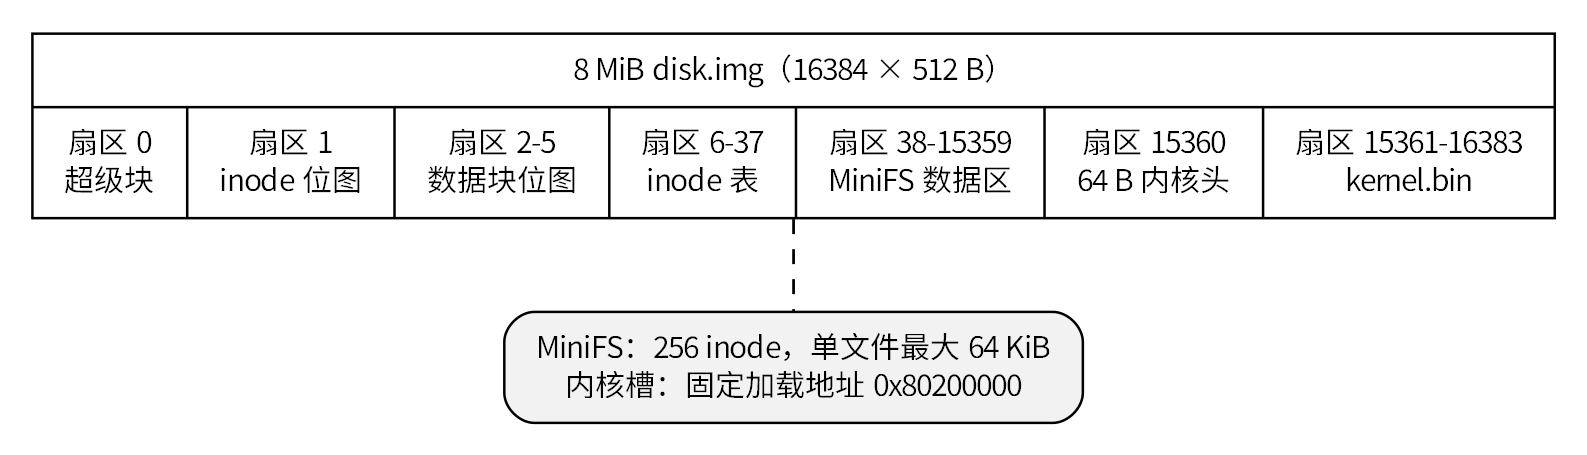
\includegraphics[width=0.94\linewidth,height=0.78\textheight,keepaspectratio]{figures/fig06_disk.png}
\caption{MiniFS v2 磁盘布局图}
\end{figure}
\end{landscape}

\section{inode 与目录项}

MiniFS v2 使用 inode 表示文件和目录。每个 inode 包含文件类型、大小、父目录、链接计数、直接块和一级间接块。每个 inode 包含 10 个直接块和 1 个一级间接块，文件大小限制为 64 KiB。

目录由目录项组成。目录项记录 inode 号、类型和文件名。路径解析时，文件系统从根目录或当前工作目录出发，逐级查找目录项，支持 \nolinkurl{.} 和 \nolinkurl{..}。

MiniFS v2 的 inode、目录项和路径解析均由内核直接实现：

\begin{lstlisting}[language=c]
struct minifs_inode {
    uint32_t mode, size, parent, links;
    uint32_t direct[MINIFS_DIRECT_BLOCKS];
    uint32_t indirect;
    uint32_t reserved;
};

struct minifs_dirent {
    uint32_t inode;
    uint32_t mode;
    char name[56];
};
\end{lstlisting}

路径解析从根目录或当前工作目录开始，并显式处理 \nolinkurl{.} 和 \nolinkurl{..}。

\section{文件描述符管理}

MiniOS 采用“每进程 fd 表 + 全局 open file 表”的设计。每个进程拥有独立 fd 表，全局 open file 表保存文件偏移、引用计数、打开模式和 inode 信息。

该设计支持：

\begin{enumerate}
\item \nolinkurl{fork} 后父子进程共享 open file description。
\item \nolinkurl{execve} 时保留普通 fd。
\item close-on-exec 标志控制部分 fd 在 exec 成功后关闭。
\item \nolinkurl{dup2} 支持重定向。
\item Shell 通过 \nolinkurl{<}、\nolinkurl{>}、\nolinkurl{>>} 实现输入输出重定向。
\end{enumerate}

\section{文件系统小结}

MiniFS v2 使 MiniOS 具备了真正的持久化能力。用户可以在 Shell 中创建目录、写入文件、读取文件，并在模拟器重启后再次访问这些文件。文件系统同时也是 ELF 用户程序存储和加载的基础。

\chapter{用户程序与 Shell}

\section{ELF 用户程序}

MiniOS 的用户程序不再以内嵌汇编形式写入内核，而是作为独立 ELF64 RISC-V 静态程序存储在 MiniFS 中。内核通过 ELF loader 加载用户程序，并通过 \nolinkurl{sret} 进入 U 态执行。

用户程序包括：

\begin{lstlisting}
/bin:
shell ls cat echo pwd ps kill env mkdir rm touch write

/tests:
spin fstest forktest argtest
\end{lstlisting}

\section{用户程序启动入口}

每个用户程序通过 \nolinkurl{crt0.S} 启动。\nolinkurl{crt0.S} 从用户栈中解析 \nolinkurl{argc/argv/envp}，然后调用 C 语言 \nolinkurl{main} 函数。当 \nolinkurl{main} 返回后，用户程序通过 \nolinkurl{exit} 系统调用退出。

\nolinkurl{os/user/crt0.S} 的用户程序入口如下：

\begin{lstlisting}
_start:
    ld a0, 0(sp)       # argc
    addi a1, sp, 8     # argv
    slli t0, a0, 3
    add t0, a1, t0
    addi a2, t0, 8     # envp
    call main
    li a7, 93          # SYS_EXIT
    ecall
\end{lstlisting}

\section{Shell 功能}

Shell 是 MiniOS 的第一个用户进程，也是用户与系统交互的入口。Shell 支持：

\begin{enumerate}
\item 命令行读取。
\item 当前工作目录提示符。
\item 内建命令：\nolinkurl{help/cd/exit/exec/run}。
\item PATH 搜索。
\item 外部命令执行。
\item \nolinkurl{fork + execve}。
\item 前台进程等待。
\item 后台进程运行。
\item 输入输出重定向。
\item \nolinkurl{ps/kill} 进程管理。
\end{enumerate}

Shell 执行外部命令的典型流程为：

\begin{lstlisting}
读取命令
  -> 解析 argv、重定向和后台标志
  -> fork
      -> 子进程处理重定向
      -> execve 加载目标 ELF
      -> 新程序进入 U 态运行
  -> 父进程根据前台/后台决定 waitpid 或继续读取命令
\end{lstlisting}

\reportfigure{fig07_shell.png}{0.55}{Shell fork/execve 用户程序执行链路图}

\nolinkurl{os/user/shell.c} 执行外部命令的核心逻辑如下：

\begin{lstlisting}[language=c]
int pid = fork();
if (pid == 0) {
    if (apply_redirections(&shell_command) < 0)
        exit(126);
    if (try_exec(program_argv, envp) < 0)
        exit(127);
}
if (shell_command.background)
    printf("[pid %d]\n", pid);
else
    wait_for(pid);
\end{lstlisting}

\chapter{系统运行与功能测试}

\section{构建方式}

项目主要构建命令如下：

\begin{lstlisting}[language=bash]
# 构建模拟器和单元测试
cmake --build build_wsl -j$(nproc)

# 构建 MiniOS 内核和用户程序
cd os
make

# 重新生成磁盘镜像
make disk FORCE=1

# 运行 MiniOS
make run
\end{lstlisting}

也可以使用无颜色构建，方便测试脚本匹配输出：

\begin{lstlisting}[language=bash]
cd os
make clean && make BOOT_COLOR=0
make disk FORCE=1
make run
\end{lstlisting}

\section{已完成的底层单元测试}

当前项目包含较多面向模拟器和硬件抽象的自动化测试，用于验证 MiniOS 所依赖的底层平台正确性。测试覆盖：

\begin{table}[H]
\centering
\small
\begin{adjustbox}{max width=\textwidth}
\begin{tabularx}{\textwidth}{>{\raggedright\arraybackslash}X>{\raggedright\arraybackslash}X}
\toprule
\textbf{类别} & \textbf{说明} \\
\midrule
RV 指令测试 & 验证 RV64I 指令实现 \\
CSR 测试 & 验证控制状态寄存器读写和委托逻辑 \\
DRAM 测试 & 验证主存读写 \\
Bus 测试 & 验证地址路由与 MMIO \\
CPU 测试 & 验证 CPU 执行流程 \\
Exception 测试 & 验证异常建模 \\
PLIC 测试 & 验证外部中断控制器 \\
CLINT 测试 & 验证定时器 \\
UART 测试 & 验证串口输入输出 \\
MMU 测试 & 验证 Sv39 地址翻译和权限检查 \\
mkfs 测试 & 验证 MiniFS 镜像构建工具 \\
install-kernel 测试 & 验证内核安装和磁盘迁移工具 \\
\bottomrule
\end{tabularx}
\end{adjustbox}
\end{table}

2026 年 6 月 20 日执行：

\begin{lstlisting}[language=bash]
ctest --test-dir build_wsl --output-on-failure
\end{lstlisting}

结果为 \textbf{99/99 项 CTest 全部通过}。其中包含 96 项 C++/GoogleTest 测试、\nolinkurl{mkfs_minifs} 与 \nolinkurl{install_kernel} 两项 Python 工具测试，以及一项 \nolinkurl{minios_integration} 系统级测试。该部分测试证明 \nolinkurl{cemu}、镜像制作工具和 MiniOS 完整运行链路均可通过统一命令回归验证。

\section{MiniOS 手动运行验证}

MiniOS 当前已经通过以下运行流程验证：

\begin{enumerate}
\item Bootloader 从磁盘加载内核。
\item 内核进入 S 态。
\item 物理内存初始化成功。
\item Sv39 虚拟内存初始化成功。
\item MiniFS v2 挂载成功。
\item 调度器初始化成功。
\item 用户 Shell 启动成功。
\item Shell 能接收命令。
\item Shell 退出后系统能主动停机。
\end{enumerate}

典型启动输出如下：

\begin{lstlisting}
[BOOT] MiniOS loader
[BOOT] reading kernel header
[BOOT] loading kernel -> 0x0000000080200000
[BOOT] checksum OK
[BOOT] jumping to kernel 0x0000000080200000

MiniOS | RV64I | S-mode | Sv39

[ OK ] Physical memory
[ OK ] Virtual memory
[ OK ] MiniFS
[ OK ] Scheduler
[ OK ] User shell

Welcome to MiniOS.
Type 'help' for commands.
minios:/>
\end{lstlisting}

\reportfigure{fig08_terminal.png}{0.90}{MiniOS 启动到 Shell 的终端界面}

\section{MiniOS 系统级自动化测试}

为了避免测试只集中在模拟器模块，本项目已经实现 \nolinkurl{tests/test_minios_integration.py} 系统级集成测试框架。该框架以完整操作系统行为为对象，而不是只测试某个内核函数或硬件模块。

测试框架的实现方式如下：

\begin{enumerate}
\item 使用 Python 启动 \nolinkurl{cemu}。
\item 加载 \nolinkurl{os/build/boot.bin}。
\item 使用临时复制的 \nolinkurl{disk.img}，避免破坏正式磁盘。
\item 通过 stdin 向 Shell 输入命令。
\item 收集 stdout 输出。
\item 使用关键字符串和正则表达式判断测试是否通过。
\item 每次等待设置 20 秒超时，避免模拟器或 Shell 卡死。
\item 普通用例为每个测试复制独立临时磁盘；持久化用例则故意复用同一临时磁盘并连续启动两次。
\item 测试结束后检查 \nolinkurl{cemu} 是否正常退出，并清理临时文件和子进程。
\end{enumerate}

执行命令：

\begin{lstlisting}[language=bash]
python3 tests/test_minios_integration.py
\end{lstlisting}

2026 年 6 月 20 日实测结果为：

\begin{lstlisting}
Ran 7 tests in 4.385s

OK
\end{lstlisting}

因此，当前仓库的自动化验证应准确表述为：

\begin{lstlisting}
99 项 CTest 测试项，其中 minios_integration 内部执行 7 个系统级用例
\end{lstlisting}

底层计数仍可理解为 96 项 C++ 单元测试、2 项 Python 工具测试和 7 项系统级用例，共 105 个自动化检查；但在 CTest 输出中，7 项系统级用例被封装为一个 \nolinkurl{minios_integration} 测试项，因此 CTest 显示总数为 99。

\section{已实现的系统级集成测试用例}

\subsection{启动与 Shell 测试}

输入命令：

\begin{lstlisting}
help
exit
\end{lstlisting}

实际验证：

\begin{enumerate}
\item 系统成功启动到 Shell。
\item Shell 输出帮助信息。
\item Shell 可以正常退出。
\item 内核可以主动停机。
\end{enumerate}

主要断言：

\begin{lstlisting}
Welcome to MiniOS
minios:/>
Built-in commands
Shell exited
\end{lstlisting}

\subsection{文件系统基础测试}

输入命令：

\begin{lstlisting}
mkdir /tmp/demo
write /tmp/demo/message.txt hello
cat /tmp/demo/message.txt
ls /tmp/demo
exit
\end{lstlisting}

实际验证：

\begin{enumerate}
\item 可以创建目录。
\item 可以创建并写入普通文件。
\item 可以读取文件内容。
\item 可以列出目录项。
\end{enumerate}

主要断言：

\begin{lstlisting}
hello
message.txt
\end{lstlisting}

\subsection{ELF 用户程序与参数测试}

输入命令：

\begin{lstlisting}
argtest hello "two words"
exit
\end{lstlisting}

实际验证：

\begin{enumerate}
\item Shell 能够执行 \nolinkurl{/tests/argtest}。
\item \nolinkurl{execve} 能够加载 ELF 用户程序。
\item 用户栈中的 \nolinkurl{argc/argv} 构造正确。
\item 引号参数能够被正确解析。
\end{enumerate}

主要断言：

\begin{lstlisting}
argc
hello
two words
\end{lstlisting}

当前脚本实际匹配 \nolinkurl{argc}、\nolinkurl{hello} 和 \nolinkurl{two words}，与 \nolinkurl{argtest} 的真实输出一致。

\subsection{fork / exec / wait 测试}

输入命令：

\begin{lstlisting}
forktest
exit
\end{lstlisting}

实际验证：

\begin{enumerate}
\item \nolinkurl{fork} 能创建子进程。
\item 子进程可以 \nolinkurl{execve} 执行新程序。
\item 父进程可以 \nolinkurl{waitpid} 等待子进程。
\item 子进程退出码能够被正确回收。
\end{enumerate}

主要断言：

\begin{lstlisting}
PASS
\end{lstlisting}

\subsection{文件系统压力测试}

输入命令：

\begin{lstlisting}
fstest
exit
\end{lstlisting}

实际验证：

\begin{enumerate}
\item MiniFS 能进行文件读写。
\item 支持 seek。
\item 支持较大文件和间接块。
\item 文件内容校验正确。
\end{enumerate}

主要断言：

\begin{lstlisting}
PASS
\end{lstlisting}

\subsection{后台进程、ps 与 kill 测试}

输入命令：

\begin{lstlisting}
spin &
ps
kill -15 <PID>
exit
\end{lstlisting}

测试脚本需要从 \nolinkurl{[pid N]} 输出中提取后台进程 PID，然后自动发送 \nolinkurl{kill -15 N}。

实际验证：

\begin{enumerate}
\item Shell 支持后台进程。
\item \nolinkurl{ps} 能显示进程状态。
\item \nolinkurl{kill -15 PID} 调用后 Shell 能重新返回提示符。
\item 后台进程不会阻塞 Shell，系统仍能正常退出。
\end{enumerate}

主要断言：

\begin{lstlisting}
[pid N]
spin
\end{lstlisting}

\subsection{持久化测试}

第一次启动输入：

\begin{lstlisting}
mkdir /tmp/persist
write /tmp/persist/data.txt persistent
exit
\end{lstlisting}

第二次使用同一个临时磁盘再次启动，输入：

\begin{lstlisting}
cat /tmp/persist/data.txt
exit
\end{lstlisting}

实际验证：

\begin{enumerate}
\item 文件内容写入磁盘镜像。
\item 模拟器重启后文件仍然存在。
\item MiniFS v2 具有持久化能力。
\end{enumerate}

主要断言：

\begin{lstlisting}
persistent
\end{lstlisting}

\section{测试结果小结}

通过上述测试设计，MiniOS 的验证体系可以分为两层：

第一层是模拟器和硬件抽象单元测试，证明 CPU、CSR、MMU、Bus 和外设模型正确。

第二层是 7 项 MiniOS 系统级集成测试，证明 Bootloader、内核、Shell、进程、文件系统、ELF loader 和系统调用能够形成完整操作系统闭环。

两层测试在 2026 年 6 月 20 日均已实际通过。7 项系统测试已经以 \nolinkurl{minios_integration} 名称注册到 CTest，并设置 180 秒超时和串行执行属性，因此一条 \nolinkurl{ctest} 命令即可统一运行全部回归测试。

\chapter{项目特色与扩展}

\section{自研 RISC-V 模拟平台与操作系统协同验证}

题目允许直接使用 QEMU、Bochs 等现成模拟器，本项目则将前序课程中开发的 RV64I 模拟器扩展为 MiniOS 的运行平台。CPU、CSR、MMU、Bus、CLINT、PLIC、UART 和块设备均可在源码层追踪，使一次用户命令能够沿着 Shell、系统调用、页表翻译、总线和设备模型逐层分析。

该特色不在于“没有使用 QEMU”本身，而在于形成了可控制、可调试、可进行跨层验证的软硬件协同实验环境。

\section{启动镜像与持久化文件系统的协同磁盘设计}

MiniFS v2 和 Bootloader 共用一个 8 MiB \nolinkurl{disk.img}：前部为持久化文件系统，尾部为带镜像头和 checksum 的内核槽。配套工具可以安全安装内核、检查镜像大小，并在尾部未被占用时迁移旧版磁盘布局。

独立 Bootloader 和持久化文件系统分别属于课程功能要求；将两者组织在同一磁盘布局中，并提供校验、更新和兼容迁移工具，是本项目额外完成的工程化设计。

\section{从硬件单元测试到系统行为的统一回归验证}

项目不仅验证单个 CPU、CSR、MMU 和外设模块，还通过真实 Shell 交互测试启动、文件操作、ELF 参数、\nolinkurl{fork/exec/wait}、后台进程和跨重启持久化。每个系统测试使用临时磁盘副本，既避免污染正式镜像，也能稳定复现测试结果。

7 个系统级用例已封装为 CTest 中的 \nolinkurl{minios_integration} 测试项，与其他 98 项测试统一执行。该测试体系属于题目功能验收之外的工程质量扩展。

\chapter{当前不足}

虽然 MiniOS 已经形成教学操作系统闭环，但仍存在一些不足：

\begin{enumerate}
\item \textbf{未适配 QEMU}：当前系统运行在自研 \nolinkurl{cemu} 上，尚未证明能够直接在 QEMU \nolinkurl{virt} 平台启动。
\item \textbf{未实现完整 Demand Paging}：当前支持 Sv39 和用户地址空间，但尚未实现 ELF 段懒加载、缺页修复、栈自动增长和换页机制。
\item \textbf{Shell 不支持管道}：当前 Shell 支持重定向和后台任务，但尚未实现 \nolinkurl{cmd1 | cmd2} 形式的管道。
\item \textbf{UART 输入主要采用轮询方式}：当前可以完成终端输入输出，但尚未实现完整的 UART RX 中断输入路径。
\item \textbf{用户权限模型不完整}：当前文件系统没有实现多用户权限模型，也没有完整的用户组、权限位和访问控制。
\item \textbf{文件系统没有日志机制}：MiniFS v2 能持久化保存数据，但不支持日志和异常断电恢复。
\item \textbf{用户异常隔离测试仍需补充}：当前已统一运行底层和系统级测试，但尚缺少非法指令、用户态缺页等异常仅终止故障进程且不影响 Shell 的自动化测试。
\end{enumerate}

\chapter{总结与展望}

\section{项目总结}

本项目完成了一个运行在自研 RV64I 模拟平台上的教学型操作系统 MiniOS。系统实现了从 Bootloader 到用户态 Shell 的完整链路，支持 M/S/U 特权级、Sv39 虚拟内存、进程管理、时间片调度、系统调用、MiniFS v2 文件系统、ELF 用户程序和交互式 Shell。

与简单的内核 demo 相比，MiniOS 已经具备较完整的操作系统形态。用户可以通过 Shell 创建文件、读取文件、执行程序、启动后台任务、查看进程、终止进程，并验证文件跨模拟器重启持久保存。

本项目最核心的价值在于打通了以下链路：

\begin{lstlisting}
Bootloader
  -> S-mode Kernel
  -> Trap / Syscall
  -> Scheduler
  -> MiniFS
  -> ELF Loader
  -> User Program
  -> Shell
\end{lstlisting}

这条链路展示了操作系统从启动、内核管理到用户程序执行的完整过程。

\section{后续展望}

后续可以从以下方向继续完善：

\begin{enumerate}
\item 实现用户态 page fault 隔离和 lazy stack。
\item 实现更完整的 Demand Paging。
\item 实现 Shell 管道。
\item 实现 UART 中断输入。
\item 增加用户态同步机制和资源竞争测试。
\item 补充用户异常隔离测试，并修复集成测试退出时偶发的 Python \nolinkurl{ResourceWarning}。
\item 增加文件系统日志机制。
\item 适配 QEMU \nolinkurl{virt} 平台。
\item 增加更多用户程序。
\item 改进内核堆分配器，实现字节级 \nolinkurl{kmalloc/kfree}。
\end{enumerate}

\section{结语}

通过本次课程设计，我对操作系统的理解从教材中的模块概念推进到了工程实现层面。系统启动、特权级切换、trap、系统调用、进程调度、虚拟内存、文件系统和用户程序并不是孤立知识点，而是互相依赖、共同构成操作系统运行闭环的组件。

MiniOS 仍然是一个教学型系统，距离成熟操作系统还有很大差距，但它已经能够完整展示“一个用户命令如何从 Shell 出发，经过内核机制，最终访问文件系统并返回结果”的全过程。这也是本项目最重要的实现成果。

\appendix
\chapter*{附录：项目完成度对照表}
\addcontentsline{toc}{chapter}{附录：项目完成度对照表}

\small
\begin{longtable}{>{\raggedright\arraybackslash}p{0.10\textwidth}>{\raggedright\arraybackslash}p{0.15\textwidth}>{\raggedright\arraybackslash}p{0.30\textwidth}>{\raggedright\arraybackslash}p{0.08\textwidth}>{\raggedright\arraybackslash}p{0.17\textwidth}}
\caption{项目完成度对照表}\label{tab:completion}\\
\toprule
\textbf{课程模块} & \textbf{课程主要要求} & \textbf{本项目完成内容} & \textbf{状态} & \textbf{主要差距} \\
\midrule
\endfirsthead
\multicolumn{5}{c}{\small 表 \thetable\ 项目完成度对照表（续）}\\
\toprule
\textbf{课程模块} & \textbf{课程主要要求} & \textbf{本项目完成内容} & \textbf{状态} & \textbf{主要差距} \\
\midrule
\endhead
\midrule
\multicolumn{5}{r}{\small 接下页}\\
\endfoot
\bottomrule
\endlastfoot
系统启动 & 特权级切换、加载内核、初始化 Trap 与栈、输出日志 & 实现独立 Bootloader，从磁盘校验并加载内核，完成 M→S 切换和稳定启动 & 完成 & 尚未适配 QEMU \nolinkurl{virt} \\
中断与异常 & 中断入口、时钟与输入中断、系统调用、缺页异常 & 实现 Trap 保存恢复、约 100 Hz 时钟中断、\nolinkurl{ecall} 系统调用；模拟器可产生页异常 & 部分完成 & UART 输入仍以轮询为主；内核未实现缺页修复和用户异常隔离 \\
内存管理 & 物理页分配、虚拟内存、内核堆、用户地址空间、按需分页 & 实现 4 KiB 页分配与复用、Sv39、独立用户页表、ELF 段和用户栈 & 部分完成 & 未实现字节级 \nolinkurl{kmalloc/kfree} 和 Demand Paging \\
进程管理 & PCB、\nolinkurl{fork/exec}、FCFS/RR、进程状态、同步、\nolinkurl{wait} & 实现 PCB、FCFS/RR、READY/RUNNING/BLOCKED/ZOMBIE、\nolinkurl{fork/execve/exit/wait/waitpid}、信号量和互斥锁 & 完成 & 未在 QEMU 环境单独测量切换开销 \\
文件系统 & 文件与目录、fd、路径、重定向、128 文件、64 KiB、seek、mkfs & 实现持久化 MiniFS v2、256 inode、多级目录、fd 表、重定向、seek 和 mkfs 工具 & 完成 & 没有日志和异常断电恢复机制 \\
用户程序 & ELF、用户栈、libc、Shell、至少 5 个程序、参数和管道 & 实现 ELF64 loader、\nolinkurl{argc/argv/envp}、简化 libc、Shell、12 个命令和 4 个测试程序 & 部分完成 & Shell 尚不支持管道；缺少用户程序崩溃隔离测试 \\
\end{longtable}
\normalsize

\end{document}
